\subsection{STAR}

Derivado de CenSurE(\emph{Center Surround Extrema}), STAR\cite{STAR}, assim como
SURF citado na Se��o~\ref{sec:surf} � baseado em \emph{box filters}. Entretanto,
enquanto DoB n�o � invariante � rota��o, � introduzido o filtro
\emph{center surround} que s�o bi-level. A Figura~\ref{fig:bilevelfilter} mostra
o padr�o do filtro bi-level em v�rios n�veis, sendo o quanto mais circular, mais
preciso, entretanto tamb�m mais dif�cil de se calcular.
 
\begin{figure}[H]
\centering
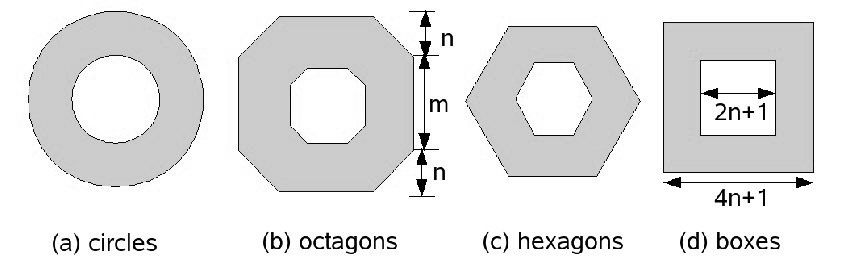
\includegraphics[scale=0.6]{images/bilevelfilter}
\caption{Filtro bi-level aplicado � formas de n lados. Fonte \cite{STAR}}
\label{fig:bilevelfilter}
\end{figure}


O detector de caracter�sticas de STAR em contrapartida � proposta do CenSurE,
usa um filtro composto de dois quadrados rotacionados. A resposta do filtro � calculada para sete escalas em cada pixel
da Figura. Em contraste com SIFT e SURF, o tamanho da amostra � constante em
cada escala e tende � resolu��o total em cada escala.
Um passo de p�s processamento � realizado para suprimir os n�o m�ximos e as
linhas.
Caracter�sticas que est�o ao longo de linhas s�o detectadas devido � matriz de
gradientes, como apresentado na equa��o~\ref{eq:gftt}.

